\chapter{Logica per Agenti}

La logica è stata sviluppata nel corso di molti secoli da matematici e filosofi per modellare il "ragionamento corretto" degli esseri umani e ha avuto un ruolo importante nello sviluppo dell'intelligenza artificiale per realizzare agenti e sistemi multiagente.

\paragraph{La logica fornisce strumenti formali per:}

\begin{itemize}
  \item \fancyglitter{La rappresentazione della conoscenza}: 
    \begin{itemize}
      \item Un linguaggio formale con una semantica precisa. 
      \item Rappresentazione dichiarativa della conoscenza.
    \end{itemize}
  \item \fancyglitter{Ragionamento automatico}:
    \begin{itemize}
      \item Refole di inferenza.
    \end{itemize}
\end{itemize}

\nt{Queste proprietà della logica hanno diverse qualità: per esempio possono spiegare in modo preciso i passi di ragionamento di un agente.}

\paragraph{Ruoli della logica per gli agenti:}

\begin{itemize}
  \item La logica può essere utilizzata da un agente intelligente per \fancyglitter{rappresentare la conoscenza} e per \fancyglitter{ragionare}. Dato che la conoscenza è espressa in un linguaggio formale, gli agenti possono usare metodi formali per derivare altra conoscenza. 
  \item La logica può servire per \fancyglitter{specificare il comportamento} di un agente intelligente. In questo caso la logica può essere usata per \fancyglitter{verificare} che l'agente si comporti come specificato, anche se l'agente non fa uso della logica nel suo funzionamento.
\end{itemize}

\paragraph{La logica classica:}

\begin{itemize}
  \item Normalmente, quando si parla di logica in ambito AI si intende la \fancyglitter{logica classica}, ossia la \fancyglitter{logica proposizionale} o la \fancyglitter{logica del primordine}. 
  \item Però la necessità di modellare concetti diversi e le esigenze di efficienza hanno portato l'AI all'uso di logiche diverse da quelle classiche e anche alla definizione di nuove logica, per esempio le logiche non monotone. 
  \item Nell'ambito degli agenti e dei sistemi multiagente si preferisce utilizzare la \fancyglitter{logica modale}.
\end{itemize}

\section{Richiami di Logica Classica}

\dfn{Logica Classica}{
  Le formule sono costituite da proposizioni atomiche appartenenti a un insieme $P$ e da connettivi logici secondo la seguente formulazione, con $p \in P, \phi, \psi$ sono formule:
  \begin{itemize}
    \item $p$. 
    \item $\phi \lor \psi$. 
    \item $\neg \phi$.
  \end{itemize}
}

\nt{Quelli presentati nella definizione sono solo alcuni dei connettivi (ci sono anche and, nand, nor, xor, implica, etc.).}
\subsection{Semantica}
\dfn{Semantica della Logica Proposizionale}{
  La semantica definisce la verità delle formule rispetto a ogni modello. Nella logica proposizionale, un modello  assegna un valore di verità (true o false) a ogni simbolo proposizionale.
}

\clm{}{}{
  \begin{itemize}
    \item Se $|P| = n$ ci sono $n$ modelli (tavole di verità). 
    \item Un modello può essere rappresentato come un insieme $M \subseteq P$ che contiene tutte le proposizioni atomiche che sono vere nel modello. Quelle che non appartengono a $M$ sono false.
  \end{itemize}
}

\dfn{Soddisfacibilità}{
  La semantica definisce una relazione di soddisfacibilità $M \vDash \phi$ di una formula $\phi$ in un modello $M$ (interpetazione):
  \begin{itemize}
    \item $M \vDash p$ se e solo se $p \in M$. 
    \item $M \vDash \phi \lor \psi$ se e solo se $M \vDash \phi$ o $M \vDash \psi$. 
    \item $M \vDash \neg \phi$ se e solo se $M \not \vDash \phi$. 
  \end{itemize}
}

\clm{}{}{
  \begin{itemize}
    \item Una formula è \fancyglitter{soddisfacibile} se è solo se c'è \fancyglitter{qualche} modlelo che la soddisfa. 
    \item Una formula è \fancyglitter{valida} se e solo se è soddisfatta da \fancyglitter{ogni modello} (tautologia).
  \end{itemize}
}

\subsection{Sistemi Deduttivi e Logica del Primordine}

\dfn{Modus Ponens}{
  $$\frac{\alpha \Rightarrow \beta \:\:\:\:\:\: \alpha}{\beta}$$
}

\nt{L'applicazione di una sequenza di regole di inferenza porta a una derivazione $KB \vdash \alpha$. Ovviamente ciò che si deriva da un insieme $KB$ è vero in tutti i modelli di $KB$.}

\dfn{Deduzione}{
  Data una base di conoscenza (insieme di formule) da $KB$, una formula $\alpha$ segue logicamente da $KB$: 
$$KB \vDash \alpha$$
se e solo se, in ogni modello in cui $KB$ è vera, anche $\alpha$ lo è.
}

\cor{Teorema di Deduzione}{
  Date due formule $\alpha$ e $\beta$, 
$$\alpha \vDash \beta$$ 
se e solo se la formula 
$$\alpha \Rightarrow \beta$$ 
è valida.
}

\nt{La logica classica del primordine estende la logica proposizionale con quantificatori universali ed esistenziali.}

\section{La Logica Modale}

\subsection{Inadeguatezza della Logica Classica}

Gli agenti sono descritti come \fancyglitter{sistemi intenzionali} attribuendo loro \fancyglitter{stati mentali}. Supponiamo di voler formulare, con la logica, la seguente frase: \fancyglitter{John crede che Superman voli}. In logica classica questo potrebbe essere espresso come: \textit{Bel(John, vola(Superman))}, dove \textit{Bel} è un predicato. 

\paragraph{Questa formulazione non funziona per almeno due ragioni:}

\begin{itemize}
  \item \fancyglitter{Ragione sintattica}: le formule della logica classica hanno la seguente struttura \textit{Predicato(Term, \dots, Term)}, però il secondo argomento di \textit{Bel} è una formula e non un termine come richiesto. 
\item \fancyglitter{Ragione semantica}: gli operatori intenzionali come \textit{Bel}sono \fancyglitter{referentially opaque}, ossia creano contesti chiusi in cui non è possibile sostituire una formula con una equivalente come in logica classica.
\end{itemize}

\subsection{Introduzione alla Logica Modale}

La semantica della \fancyglitter{logica modale} è formulata in termini di \fancyglitter{mondi possibili}. Ogni mondo rappresenta una situazione considerata possibile dall'agente. Ciò che è vero in tutti i mondi si può dire sia creduto dall'agente.

\begin{itemize}
  \item Da un punto di vista filosofico, la proprietà fondamentale della logica modale è che tutto ciò che è vero in tutti i mondi è \fancyglitter{necessariamente} vero. Ciò che è vero in qualche mondo è \fancyglitter{possibile}.
  \item La logica modale è stata sviluppata per distinguere tra \fancyglitter{verità necessarie} e \fancyglitter{verità contingenti}.
\end{itemize}

\dfn{Logica Modale}{
  La logica modale proposizionale estende la logica classica proposizionale con due operatori
modali: $\Box$ (verità necessaria) e $\Diamond$ (verità contingente/possibile). Le formule sono:
\begin{itemize}
    \item $p$
    \item $\varphi \vee \psi$
    \item $\neg \varphi$
    \item $\Box \varphi$
    \item $\Diamond \varphi$
\end{itemize}
Dove $p \in P$ e $\varphi$ e $\psi$ sono formule della logica. 
}

\clm{}{}{
  \begin{itemize}
    \item I due operatori modali sono uno il duale dell'altro: $\Box\varphi \equiv \neg\Diamond\neg\varphi$ (se è necessario che $\varphi$ sia vera allora, indipendentemente da cosa sia, non è possibile che $\varphi$ sia falsa) e $\Diamond\varphi \equiv \neg\Box\neg\varphi$ (se è possibile che $\varphi$ sia vera allora non è vero che è falsa in tutti i mondi, poiché in \textit{almeno} un mondo è vera). 
    \item Volendo si potrebbe minimizzare l'uso della sintassi utilizzando solo uno dei due operatori.
  \end{itemize}
}

\dfn{Semantica della Logica Proposizionale}{
  \begin{itemize}
    \item Un \newfancyglitter{modello} della logica modale è dato come un insieme di mondi possibili. 
    \item Ogni \newfancyglitter{mondo} è costituito da un insieme di proposizioni che sono considerate vere in quel mondo. 
    \item La \newfancyglitter{struttura} del modello è descritta da una \newfancyglitter{relazione binaria di accessibilità} che collega coppie di mondi.
  \end{itemize}
}

\cor{Modello}{
  Un modello $M$ è una tripla $\langle W, R, L \rangle$ dove: 
  \begin{itemize}
    \item $W$ è un insieme di mondi. 
    \item $R \subseteq W x W$ è una relazione di accessibilità tra mondi. 
    \item $L: W \rightarrow 2^P$ dà l'insieme di proposizioni vere in ogni mondo in $W$.
  \end{itemize}
}

\ex{Modello}{
  \begin{itemize}
    \item $W = \{w_1, w_2, w_3, w_4, w_5\}$
    \item $R = \{ \langle w_1, w_2 \rangle, \langle w_1, w_4 \rangle, \langle w_2, w_2 \rangle,$  
    $\quad \langle w_2, w_3 \rangle, \langle w_3, w_2 \rangle, \langle w_3, w_4 \rangle,$  
    $\quad \langle w_5, w_2 \rangle, \langle w_5, w_4 \rangle, \langle w_5, w_5 \rangle \}$
    \item $L = \{ \langle w_1, \{p, q, r\} \rangle, \langle w_2, \{p\} \rangle,$  
    $\quad \langle w_3, \{p, r\} \rangle, \langle w_4, \{r\} \rangle, \langle w_5, \emptyset \rangle \}$
\end{itemize}
  \begin{center}
    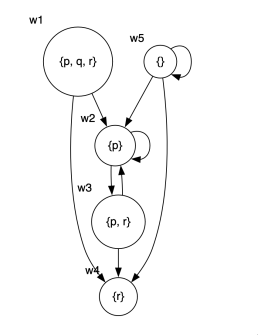
\includegraphics[scale=0.65]{02/mondi.png}
  \end{center}
  \begin{itemize}
    \item Da notare che $R$ può collegare un mondo a sé stesso con un loop.
  \end{itemize}
}

\dfn{Soddisfacibilità}{
  La soddisfacibilità di una formula $\varphi$ è definita rispetto a un modello $M$ e a un mondo $w$
di questo modello con la notazione $M \models_w \varphi$:

\begin{itemize}
    \item $M \models_w p \quad \text{se e solo se} \quad p \in L(w)$
    \item $M \models_w \varphi \vee \psi \quad \text{se e solo se} \quad M \models_w \varphi \text{ or } M \models_w \psi$
    \item $M \models_w \neg \varphi \quad \text{se e solo se} \quad M \not\models_w \varphi$
    \item $M \models_w \Box \varphi \quad \text{se e solo se} \quad \forall w' \, (R(w, w') \Rightarrow M \models_{w'} \varphi)$
    \item $M \models_w \Diamond \varphi \quad \text{se e solo se} \quad \exists w' \, (R(w, w') \Rightarrow M \models_{w'} \varphi)$
\end{itemize}

}

\cor{Validità}{
  Una formula $\varphi$ è valida se è vera in tutte le coppie modello/mondo. La nozione di validità è analoga a quella di tautologia (qualcosa che è sempre vero) nella logica proposizionale classica.
}

\nt{I modelli della logica modale sono spesso chiamati \fancyglitter{Kripke Structures}. La coppia $\langle W, R \rangle$ è chiamata \fancyglitter{Kripke frame}.}

\paragraph{Proprietà fondamentali della logica modale:}

\begin{enumerate}
  \item \fancyglitter{Assioma K}\footnote{Sempre in onore di Kripke.}: $K: \Box (\varphi \Rightarrow \psi) \leftrightarrow (\Box\varphi \Rightarrow \Box\psi)$.
  \item \fancyglitter{Necessitation}, regola di inferenza: se $\varphi$ è valida allora $\Box\varphi$ è valida. 
\end{enumerate}

\nt{L'assioma K è proprio delle logiche modali "normali". Esistono altre logiche modali che non l'hanno.}

\paragraph{Distribuitività:}

\begin{itemize}
  \item La logica modale distribuisce su AND: $\Box (\varphi \wedge \psi) \equiv (\Box \varphi \wedge \Box \psi)$. 
  \item La logica modale non distribuisce su OR: $\Box (\varphi \vee \psi) \not\equiv (\Box \varphi \vee \Box \psi)$. 

\end{itemize}

\qs{}{Ma cosa c'entra questa logica con gli agenti?}

\begin{itemize}
  \item Si dà agli operatori modali un significato diverso da quello standard (necessario o possibile) per modellare una proprietà degli agenti, senza modificare la semantica dei mondi possibili. 
  \item Si attribuisce all'operatore $\Box$ il significato di \fancyglitter{credere} (belief), ergo $\Box\varphi$ significa che l'agente crede che $\varphi$ sia vero. 
  \item Per chiarezza l'operatore $\Box$ è chiamato B (ossia belief, credenza). All'operatore duale non viene attribuito un nome.
\end{itemize}

\paragraph{Principali logiche modali per agenti:}

\begin{itemize}
  \item \fancyglitter{Logica epistemica} (conoscenza e credenza):
    \begin{itemize}
      \item $K_a\varphi$ l'agente $a$ sa che $\varphi$ è vero. 
      \item $B_a\varphi$ l'agente $a$ crede che $\varphi$ sia vero.
    \end{itemize}
  \item \fancyglitter{Logiche Belief-Desire-Intention}:
    \begin{itemize}
      \item $B_a\varphi$ l'agente $a$ crede che $\varphi$ sia vero.
      \item $D_a\varphi$ l'agente $a$ desidera $\varphi$. 
      \item $I_a\varphi$ l'agente $a$ ha l'intenzione $\varphi$.
    \end{itemize}
  \item \fancyglitter{Logiche deontologiche}:
    \begin{itemize}
      \item $O\varphi$ è obbligatorio che $\varphi$. 
      \item $P\varphi$ è permesso che $\varphi$.
    \end{itemize}
  \item \fancyglitter{Logica temporale} (lineare):
    \begin{itemize}
      \item $X\varphi$, $\varphi$ sarà vero al prossimo istante. 
      \item $G\varphi$, $\varphi$ sarà sempre vero. 
      \item $F\varphi$, $\varphi$ prima o poi diventerà vero. 
      \item $\psi \cup \varphi$, $\varphi$ è vero fino a quando $\varphi$ diventa vero. 
    \end{itemize}
  \item \fancyglitter{Logica dinamica} (delle azioni): 
    \begin{itemize}
      \item $[\pi]\varphi$ dopo l'esecuzione del programma $\pi$, $\varphi$ è vero. 
      \item $\pi$ è un'azione complessa (programma) ottenuta combinando azioni elementari.
    \end{itemize}
\end{itemize}

\clm{}{}{
  \begin{itemize}
    \item Se $\Box$ rappresenta la conoscenza, si vuole che la logica avesse la proprietà  che tutto ciò che è conosciuto è vero. Questo può essere espresso aggiungendo l'assioma:
          \[
          \Box \varphi \Rightarrow \varphi
          \]
    \item La formula $\Box \varphi \Rightarrow \varphi$ non vale in tutti i modelli.
    \item Si è può esprimere che le conoscenze dell'agente non devono essere contraddittorie,  
          aggiungendo l'assioma:
          \[
          \Box \varphi \Rightarrow \neg \Box \neg \varphi
          \]
\end{itemize}
}

\paragraph{Proprietà dei frame:}

\begin{itemize}
    \item \fancyglitter{Reflexive} ($\Box\varphi \Rightarrow \varphi$):  
          \[
          \forall w \in W \, . \, (w, w) \in R
          \]
    \item \fancyglitter{Serial} ($\Box\varphi \Rightarrow \Diamond\varphi$):  
          \[
          \forall w \in W \, . \, \exists w' \in W \, . \, (w, w') \in R
          \]
    \item \fancyglitter{Transitive} ($\Box\varphi \Rightarrow \Box\Box\varphi$):  
          \[
          \forall w, w', w'' \in W \, . \, ((w, w') \in R \wedge (w', w'') \in R) \Rightarrow (w, w'') \in R
          \]
    \item \fancyglitter{Euclidean} ($\Diamond\varphi \Rightarrow \Diamond\Diamond\varphi$):  
          \[
          \forall w, w', w'' \in W \, . \, ((w, w') \in R \wedge (w, w'') \in R) \Rightarrow (w', w'') \in R
          \]
\end{itemize}

\nt{A ciascuno di queste proprietà è stato dato un nome, in ordine: T, D, 4 e 5. Combinando queste proprietà si ottengono 11 sistemi modali (sarebbero 16, ma alcuni sono equivalenti).}

\paragraph{Ad alcuni sistemi "notevoli" è stato dato un nome:}

\begin{itemize}
  \item KT è T. 
  \item KT4 è S4. 
  \item KD45 è weak-S5.
  \item KTD45 è S5.
\end{itemize}

\begin{figure}[!h]
    \centering
    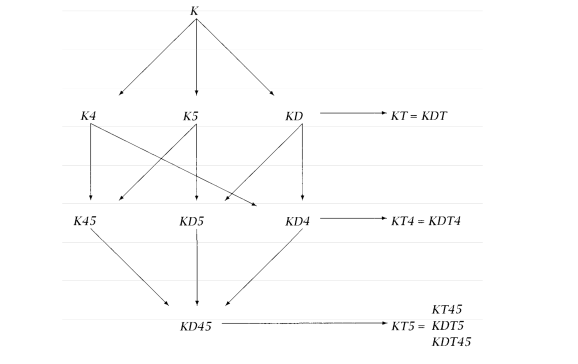
\includegraphics[scale=0.65]{02/sistemi modali.png}
    \caption{Gli 11 sistemi modali.}
\end{figure}

\section{Sistemi Modali}

\subsection{Accenni di Logica Epistemica}

\dfn{Logica Epistemica}{
La logica epistemica è la logica della conoscenza e delle credenze. Si introducono i due operatori modali $K_a$ e $B_a$ per rappresentare rispettivamente la conoscenza e le credenze di un agente.
}

\begin{itemize}
  \item \fancyglitter{Assioma K}: $K_a(\varphi\Rightarrow\psi) \leftrightarrow (K_a\varphi\Rightarrow K_a\psi)$.
  \item \fancyglitter{Necessitation}: se $\varphi$ è valida, allora $K_a\varphi$.
 
\end{itemize}

\paragraph{Il problema dell'omniscienza logica:}

\begin{itemize}
   \item Si assume che $\psi$ sia una conseguenza logica di $\varphi$. Allora $\varphi \Rightarrow \psi$ deve essere valida. Secondo la necessitation questa formula deve essere conosciuta dall'agente: $K_a(\varphi \Rightarrow \psi)$.
  \item Questo significa che l'agente deve conoscere tutte le tautologie (che sono infinite). 
  \item Inoltre se l'agente conosce $\varphi$, per l'assioma K, deve conoscere $\psi$. Questo significa che la conoscenza dell'agente è chiusa rispetto alla conseguenza logica.
  \item In altre parole se l'agente conosce una cosa e questa cosa ne implica un'altra allora l'agente deve conoscere anche quell'altra cosa.
  \item In questo corso si ignora completamente il problema.
\end{itemize}

\begin{figure}[!h]
    \centering
    
\includegraphics[scale=0.35]{02/gojo.png}
    \caption{Agente: "Throughout Heaven and Earth, I alone am the omniscient one".}
\end{figure}

\subsection{Assiomi per Knowledge e Belief}

Si possono realizzare dei sistemi modali aggiungendo nuovi assiomi alla logica modale standard: 

\begin{itemize}
  \item \fancyglitter{Assioma D (serialità):} la conoscenza di un agente è non contraddittoria, $K\varphi \Rightarrow \neg K \neg\varphi$, se l'agente conosce $\varphi$ allora non conosce $\neg\varphi$. 
  \item \fancyglitter{Assioma T (riflessività):} ciò che l'agente conosce è vero, $K\varphi\Rightarrow\varphi$, è accettabile per la conoscenza (non vogliamo che l'agente conosca qualcosa che è falso) ma non per le credenze (si accetta che l'agente creda vero qualcosa che è falso). 
  \item \fancyglitter{Assioma 4 (transitività):} $K\Rightarrow KK\varphi$.
  \item \fancyglitter{Assioma 5:} $\neg K\varphi \Rightarrow K(\neg K\varphi)$.
\end{itemize}

\nt{Gli assiomi di introspezione (4 e 5) implicano che l'agente ha conoscenza perfetta su quello che sa e quello che non sa.}

\ex{Muddy Children}{
  \begin{itemize}
    \item Consideriamo un esempio classico: dopo aver giocato nel fango, due bambini sanno  
          che almeno uno di loro ha del fango sulla fronte (in realtà tutti e due lo hanno).  
          Di solito i bambini sono almeno tre, ma per semplicità consideriamo il caso con due.  
    \item Ogni bambino può vedere la fronte dell'altro, ma non la propria.  
    \item Inizialmente il bambino B dice:  
          \[
          \text{"Non so se ho la fronte infangata"}
          \]
    \item Successivamente il bambino A dice:  
          \[
          \text{"Io so di avere la fronte infangata"}
          \]
    \item Indichiamo con $K_A$ e $K_B$ le conoscenze del bambino A e di B.    
\end{itemize}

Quindi:
\begin{enumerate}
    \item $K_A (\neg \text{muddy}(A) \Rightarrow K_B (\neg \text{muddy}(A)))$
    \item $K_A (K_B (\neg \text{muddy}(A) \Rightarrow \text{muddy}(B)))$
    \item $K_A (\neg K_B (\text{muddy}(B)))$
    \item $\neg \text{muddy}(A) \Rightarrow K_B \neg \text{muddy}(A)$, da (1) e l'assioma della conoscenza $(K \varphi \Rightarrow \varphi)$ (ciò che è conosciuto è vero)
    \item $K_B (\neg \text{muddy}(A) \Rightarrow \text{muddy}(B))$, da (2) e l'assioma della conoscenza
    \item $K_B \neg \text{muddy}(A) \Rightarrow K_B \text{muddy}(B)$, da (5) e l'assioma K $(K (\varphi \Rightarrow \psi) \Rightarrow (K \varphi \Rightarrow K \psi))$
    \item $\neg \text{muddy}(A) \Rightarrow K_B \text{muddy}(B)$, da (4) e (6) per transitività (se $\alpha \Rightarrow \beta$ e $\beta \Rightarrow \gamma$, allora $\alpha \Rightarrow \gamma$)
    \item $\neg K_B \text{muddy}(B) \Rightarrow \text{muddy}(A)$, contrapposto di (7) ($\alpha \Rightarrow \beta \equiv \neg \beta \Rightarrow \neg \alpha$)
    \item $K_A (\neg K_B \text{muddy}(B) \Rightarrow \text{muddy}(A))$, da (8) per necessitation  
          (derivazione: (1) e (2) significano che A conosce le formule (4) e (5).  
          Dalle formule (4) e (5) si deriva la formula (8), quindi (4) e (5) implicano (8) per il teorema di deduzione.  
          La regola dell'onniscienza logica implica che A conosce la formula (8))
    \item $K_A \neg K_B \text{muddy}(B) \Rightarrow K_A \text{muddy}(A)$, da (9) e l'assioma K
\end{enumerate}
}

\subsection{Ragionare sul Tempo}

La logica temporale è la logica modale del tempo. Ci sono molte varianti della logica temporale. In questo corso si tratterà solo il caso in cui il tempo: 
\begin{itemize}
  \item Ha un instante iniziale. 
  \item È infinito nel futuro.
\end{itemize}

\dfn{Linear Temporal Logic (LTL)}{
  La struttura del tempo è un insieme totalmente ordinato di istanti di tempo.  
Un modello $M$ è una struttura lineare, spesso chiamata \newfancyglitter{Kripke structure}, definita come:  

\[
M = \langle S, x, L \rangle
\]

Dove:  

\begin{itemize}
    \item $S$ è un insieme di stati.
    \item $x: \mathbb{N} \to S$ è una sequenza infinita di stati, con $\mathbb{N}$ che rappresenta l'insieme dei numeri naturali.
    \item $L: S \to 2^P$ assegna a ogni stato l'insieme delle proposizioni vere in quello stato.
\end{itemize}

}

\cor{Formule}{
  Le formule della Propositional Linear Temporal Logic (PLTL) sono definite come segue:  

\begin{itemize}
    \item $p$, con $p \in P$
    \item $\alpha \vee \beta$
    \item $\neg \alpha$
    \item $X \alpha$
    \item $\alpha U \beta$
\end{itemize}

Dove $\alpha, \beta \in$ PLTL.
}

\paragraph{Semantica informale degli operatori modali:}  

\begin{itemize}
    \item $X \alpha$ ("nexttime $\alpha$") significa che $\alpha$ è vero nel prossimo istante di tempo.
    \item $\alpha U \beta$ ("$\alpha$ until $\beta$") è vero al tempo $t$ se e solo se $\beta$ è vero in un futuro istante $t_0$ e $\alpha$ è vero in tutti gli istanti fra $t$ e $t_0$.
\end{itemize}

\paragraph{Operatori modali derivati:}  

\begin{itemize}
    \item $F \alpha \equiv \text{true} U \alpha$ ("prima o poi $\alpha$").
    \item $G \alpha \equiv \neg F \neg \alpha$ ("sempre $\alpha$").
\end{itemize}

\paragraph{In Computing Tree Logic (CTL*) è possibile formulare due tipi di formule:}

\begin{itemize}
    \item \textbf{Path formulas:} riguardano i cammini infiniti della struttura temporale ad albero e sono simili alle formule della Logica Temporale Lineare (LTL).
    \item \textbf{State formulas:} riguardano tutti i cammini infiniti uscenti da uno stato.
\end{itemize}

\qs{}{Quali sono gli usi delle logiche temporali:}

\begin{itemize}
  \item Sono usate per verificare la correttezza di sistemi concorrenti (e. g. multiagente) con la tecnica del \fancyglitter{model checking}. 
  \item Dato che il model checking affronta problemi ad alta complessità si utilizza una logica CTL (che restringe la sintassi della CTL*).
\end{itemize}

\dfn{Model Checking}{
  Il model checking è un metodo per la verifica di proprietà di agenti e di sistemi multiagente (o, in generale, sistemi concorrenti). 

}
\nt{Le proprietà da verificare sono basate su logiche temporali e sulla relazione tra i modelli delle logiche temporali e degli automi a stati finiti che ne descrivono le computazioni.}

\subsection{Ragionare sulle Azioni}

Il ragionamento sulle azioni si basa sulla logica classica: 
\begin{itemize}
  \item \fancyglitter{Situazioni}: stato del mondo a qualche istante nel tempo. 
  \item \fancyglitter{Fluenti}: proposizioni il cui valore varia da una situazione all'altra. 
  \item \fancyglitter{Azioni}: causano un cambiamento nello stato del mondo.
\end{itemize}

\dfn{Azione}{
Ogni azione è descritta da due assiomi:
\begin{itemize}
  \item Un'assioma di possibilità: che dice quando è possibile eseguire l'azione.
  \item Un'assioma di effetto: cosa accade quando un'azione possibile è eseguita.
\end{itemize}
}

\dfn{Frame Problem}{Un'azione influenza solo un numero limitato di fluenti. Bisogna trovare un modo per descrivere il fatto che tutto il resto non cambi.}

